%%
% Template for Assignment Reports
% 
%

\documentclass{article}

\usepackage{fancyhdr} % Required for custom headers
\usepackage{lastpage} % Required to determine the last page for the footer
\usepackage{extramarks} % Required for headers and footers
\usepackage{graphicx,color}
\usepackage{anysize}
\usepackage{amsmath}
\usepackage{natbib}
\usepackage{caption}
\usepackage{hyperref}
\usepackage{listings}
\usepackage{float}
\usepackage{lipsum}  
\usepackage{xcolor}
\usepackage{subcaption}

% Margins
%\topmargin=-0.45in
%\evensidemargin=0in
%\oddsidemargin=0in
\textwidth=6.5in
%\textheight=9.0in
%\headsep=0.25in 

\linespread{1.0} % Line spacing

\definecolor{codegreen}{rgb}{0,0.6,0}
\definecolor{codegray}{rgb}{0.5,0.5,0.5}
\definecolor{codepurple}{rgb}{0.58,0,0.82}
\definecolor{backcolour}{rgb}{0.95,0.95,0.92}

\lstdefinestyle{mystyle}{
    backgroundcolor=\color{backcolour},   
    commentstyle=\color{codegreen},
    keywordstyle=\color{magenta},
    numberstyle=\tiny\color{codegray},
    stringstyle=\color{codepurple},
    basicstyle=\ttfamily\footnotesize,
    breakatwhitespace=false,         
    breaklines=true,                 
    captionpos=b,                    
    keepspaces=true,                 
    numbers=left,                    
    numbersep=5pt,                  
    showspaces=false,                
    showstringspaces=false,
    showtabs=false,                  
    tabsize=2
}

\lstset{style=mystyle}

%%------------------------------------------------
%% Image and Listing code
%%------------------------------------------------
%%sw \includecode{caption for table of listings}{caption for reader}{filename}
\newcommand{\includecode}[3]{\lstinputlisting[float,floatplacement=H, caption={[#1]#2}, captionpos=b, frame=single]{#3}}


%%sw \includescalefigure{label}{short caption}{long caption}{scale}{filename}
\newcommand{\includescalefigure}[5]{
\begin{figure}[htb]
\centering
\includegraphics[width=#4\linewidth]{#5}
\captionsetup{width=.8\linewidth} 
\caption[#2]{#3}
\label{#1}
\end{figure}
}

%%sw \includefigure{label}{short caption}{long caption}{filename}
\newcommand{\includefigure}[4]{
\begin{figure}[htb]
\centering
\includegraphics{#4}
\captionsetup{width=.8\linewidth} 
\caption[#2]{#3}
\label{#1}
\end{figure}
}




%%------------------------------------------------
%% Parameters
%%------------------------------------------------
% Set up the header and footer
\pagestyle{fancy}
\lhead{\authorName} % Top left header
\chead{\moduleCode\ - \assignmentTitle} % Top center header
\rhead{\firstxmark} % Top right header
\lfoot{\lastxmark} % Bottom left footer
\cfoot{} % Bottom center footer
\rfoot{Page\ \thepage\ of\ \pageref{LastPage}} % Bottom right footer
\renewcommand\headrulewidth{0.4pt} % Size of the header rule
\renewcommand\footrulewidth{0.4pt} % Size of the footer rule
\setlength\parindent{0pt} % Removes all indentation from paragraphs

\newcommand{\assignmentTitle}{Lab 2} % Assignment title
\newcommand{\moduleCode}{CSU44061} 
\newcommand{\moduleName}{Machine Learning} 
\newcommand{\authorName}{Adriana\ Hrabowych} % Your name
\newcommand{\authorID}{19304296} % Your student ID
\newcommand{\reportDate}{\printDate}

%%------------------------------------------------
%%	Title Page
%%------------------------------------------------
\title{
\vspace{-1in}
\begin{figure}[!ht]
\flushleft

\includegraphics[width=0.4\linewidth]{reduced-trinity.png}
\end{figure}
\vspace{-0.5cm}
\hrulefill \\
\vspace{0.5cm}
\textmd{\textbf{\moduleCode\ \moduleName}}\\
\textmd{\textbf{\assignmentTitle}}\\
\vspace{0.5cm}
\hrulefill \\
}

\author{\textbf{\authorName,\ \authorID}}

\date{\today}



%%------------------------------------------------
%% Document
%%------------------------------------------------
\begin{document}
\lstset{language=Java, captionpos=b, frame=single, keywordstyle=\color{black}\bfseries, stringstyle=\ttfamily}
\captionsetup{width=.8\linewidth} 

\maketitle


%%------------------------------------------------
\section{Introduction}
In this assignment, the dataset used has the id '11-11-11'.

\section{Part i }
\begin{center}
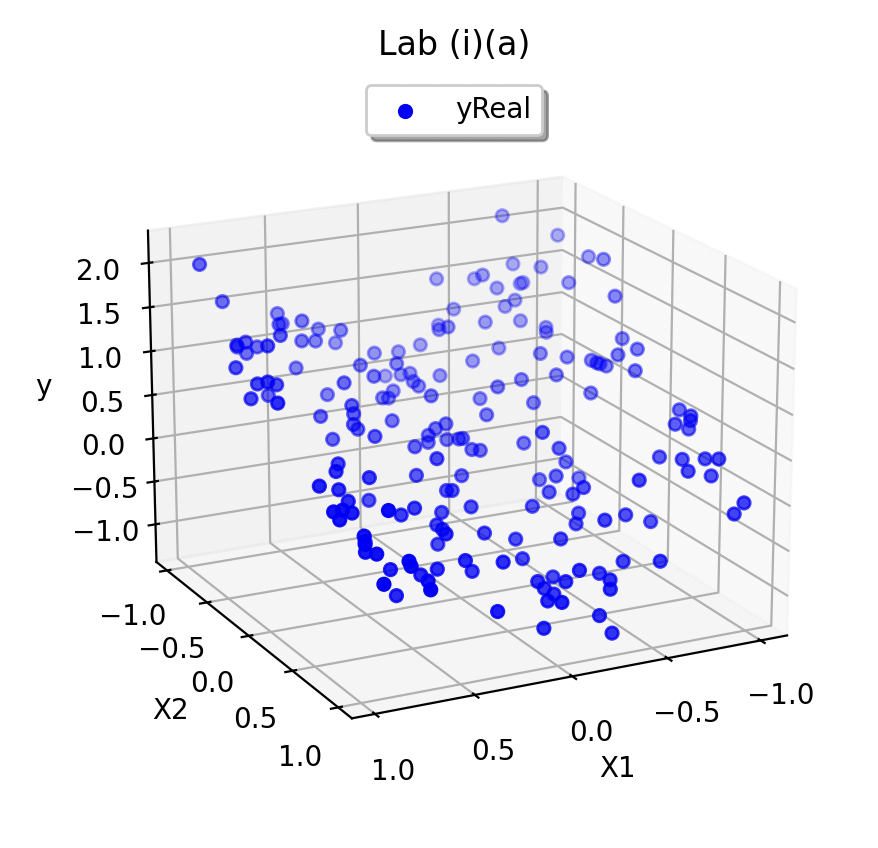
\includegraphics[width=.6\linewidth]{ia.png}
\end{center}
\captionof{figure}{A 3D scatter plot graph visualizing part A of the lab.}

\subsection{(i)(a)}
In (i)(a) the raw data is read in and organized into two arrays, one 2D array containing the two features and an 1D array containing the y valyes. Then the training data is visualized on the 3d graph seen in figure one using blue circular markers. Each data point is placed depending on the value of its two features and the target value, with the X-axis corresponding to X1, the Y-axis corresponding to X2 and the Z-axis corresponding to the target y value.

When graphed, the training data takes on the shape of a curved plane.

\subsection{(i)(b)}
As seen in section (i)(a) our data lies on a curve and as such is non linear, so in order for our models to be more accurate we need to train them with additional polynomial features. In this lab we added polynomial features up to a factor of five by using sklearn's PolynomialFeatures function. This gives us a set of 21 features made up of variations on X1 and X2 which are:

$\theta_{(1-21)} = 1, \;X_1, \;X_2, \;X_1^2, \;X_1X_2, \;X_2^2,\;X_1^3, \;X_1^2X_2, \;X_1X_2^2, \;X_2^3,\; X_1^4,\; X_1^3X_2, \;X_1^2X_2^2, \;X_1X_2^3, \;X_2^4, \;X_1^5, \;X_1^4X_2,\\ \; \mathbin{\qquad} \mathbin{\qquad} \mathbin{\qquad} \mathbin{\qquad} \mathbin{\qquad} \mathbin{\qquad}  \mathbin{\qquad} \mathbin{\quad} X_1^3X_2^2, \;X_1^2X_2^3, \;X_1X_2^4, \;X_2^5$

Now using this new set of polynomial features, four Lasso regression models were training. In Lasso, the models are linear with the addition of a cost function. The model itself is $h_\theta(x)=\theta^Tx$. The objective of the model is to minimize the cost function:
\begin{center}
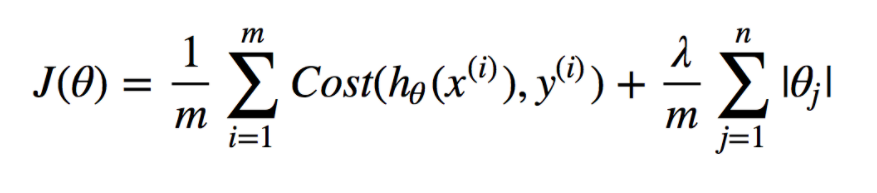
\includegraphics[width=.3\linewidth, height=1cm]{f.png}
\end{center}
Where C is a weight hyperparameter. In sklearn $\alpha$ is used instead of C, and $\alpha$ = 1/(2C)
The only difference between the four models trained is that they each have different C's: 1, 10, 100, and 1000. After training, the feature parameters were:
\begin{center}
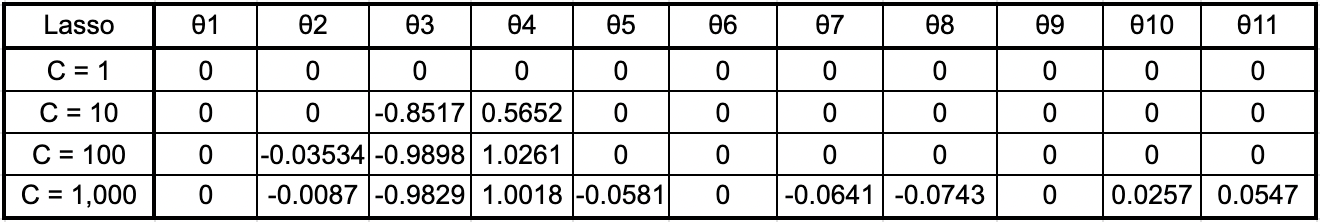
\includegraphics[width=\linewidth]{t1.png}
\caption{A table containing the Lasso feature parameters values for $\theta_1$  to  $\theta_{11}$  in the columns with each row representing a model with a different C value.}
\end{center}
\begin{center}
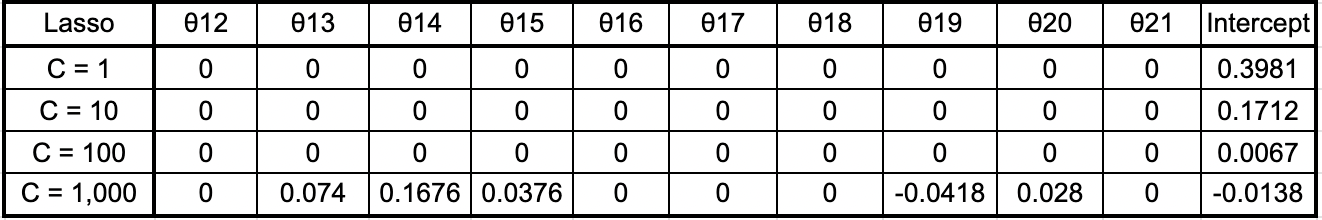
\includegraphics[width=\linewidth]{t2.png}
\caption{A table containing the Lasso feature parameters values for $\theta_12$  to  $\theta_{21}$ and the intercept in the columns with each row representing a model with a different C value.}
\end{center}

As seen in figures 2 and 3, generally as the C is raised the absolute value of each parameter also increases as the features have more influence on the predictions. The opposite is true for the intercept, which grows smaller as C increases. A lot of the feature parameters are zero as Lasso models automatically perform feature selection to eliminate the weights of less important features.

\subsection{(i)(c)}
\begin{figure}
\centering
\begin{subfigure}{.5\linewidth}
  \centering
  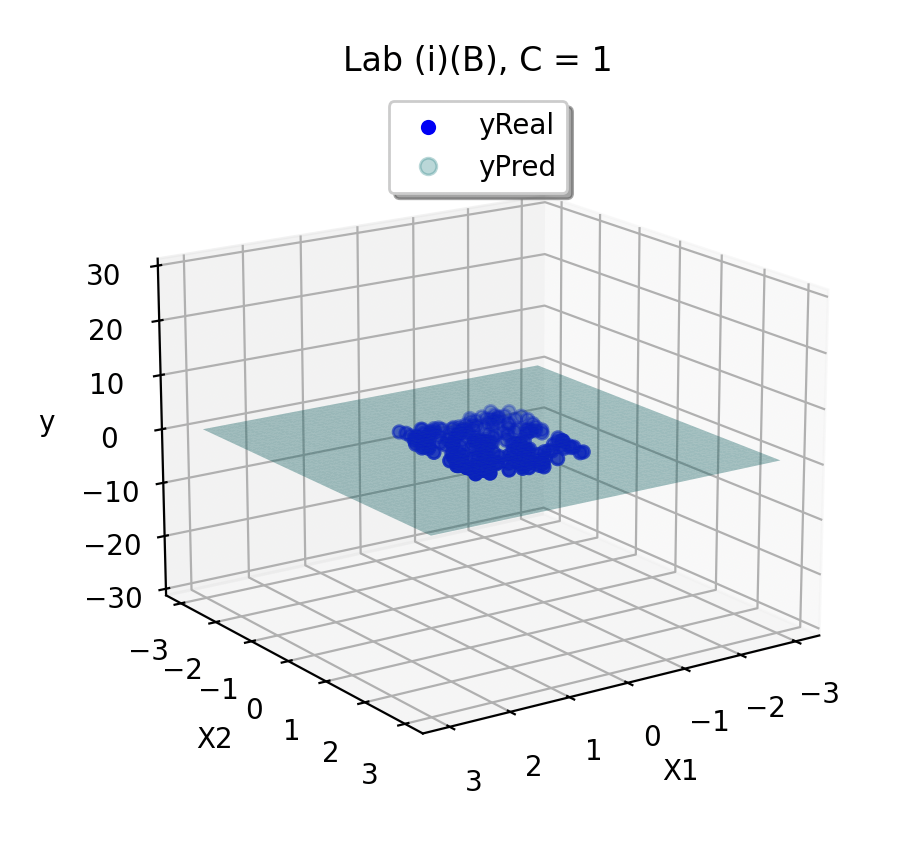
\includegraphics[width=\linewidth, height=8cm]{ib1.png}
  \caption{Lasso model predictions with C = 1}
  \label{fig:sub1}
\end{subfigure}%
\begin{subfigure}{.5\textwidth}
  \centering
  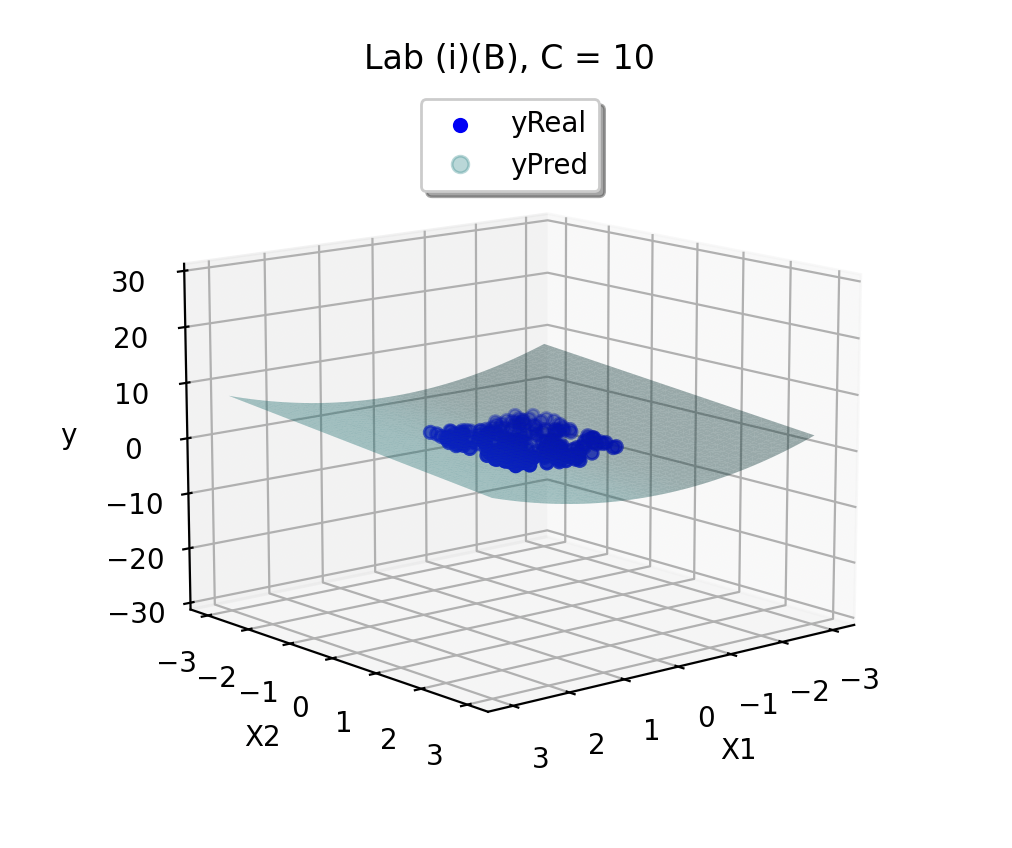
\includegraphics[width=\linewidth, height=8cm]{ib2.png}
  \caption{Lasso model predictions with C = 10}
  \label{fig:sub2}
\end{subfigure}
\label{fig:test}
\begin{subfigure}{.5\linewidth}
  \centering
  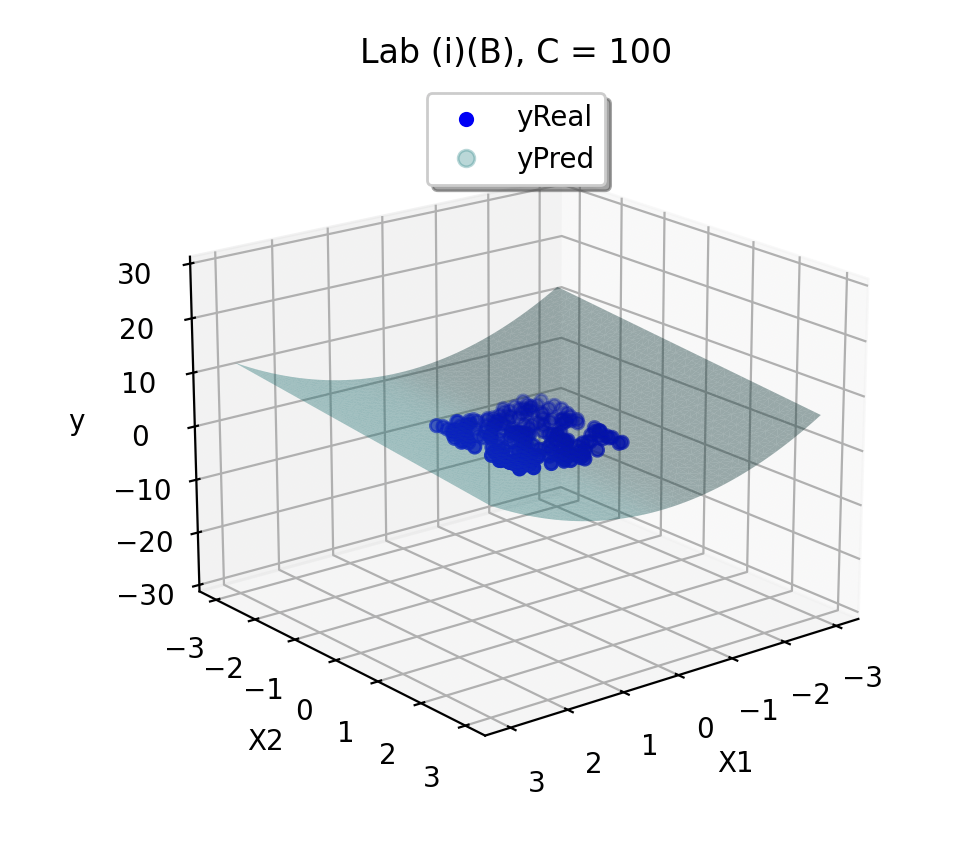
\includegraphics[width=\linewidth, height=8cm]{ib3.png}
  \caption{Lasso model predictions with C = 100}
  \label{fig:sub3}
\end{subfigure}%
\begin{subfigure}{.5\textwidth}
  \centering
  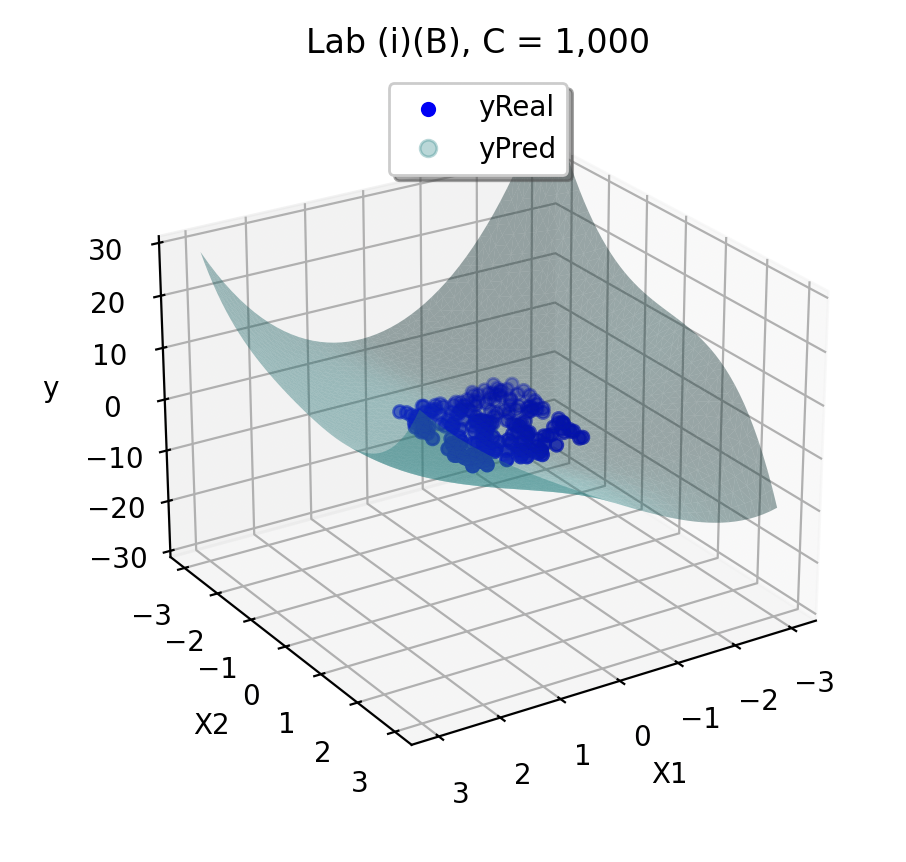
\includegraphics[width=\linewidth, height=8cm]{ib4.png}
  \caption{Lasso model predictions with C = 1,000}
  \label{fig:sub4}
\end{subfigure}
\caption{A figure with four subfigures, each containing a 3D scatter plot and plane that visualizes part ib of the lab. }
\label{fig:test}
\end{figure}

Instead of splitting our data into training and testing sections, we trained our models on all of the raw data and predict using a grid of feature values. As the original values for $X_1$ and $X_2$ were between -1 and 1, I chose to use a grid from [-3,3] as to not extend too far past the original values while still being able to see beyond the original data. The predictions are then plotted on a 3D plane.

As seen in figure 4, as C is increased the predictions begin to change from a flat linear plane (as seen when C=1) to a curved surface (seen in all other C values graphed). We originally stated that the data laid on a curved plane, so the models with higher C's seem to more accurately portray this. Though as the C gets much larger, the simple curve gives way to more complex structures.

\subsection{(i)(d)}
Underfitting is when too few features are used and as such the model cannot accurately portray the behavior of the original data. Underfit models are often incredibly inaccurate because of this. Overfitting is when too many features are used and the 'noise' in the data starts to have more influence on the predictions the model makes and as such it cannot categorize data correct.

A higher C value means the model will place a higher weight on the training data, which means that too high of a C value will cause the model to be overfit as it becomes 'overly accurate'. A lower C value puts less weight on the training data and allows more inaccuracies in predictions as it generalizes. Too low of a C can cause the lasso model to eliminate the weights of every feature parameters to 0, which causes it to be underfit. This can be seen in the graphs of figure 4, as when C=1 the surface is flat and linear and too simple to fit the data well. Whereas when C=1,000, the predicted surface becomes more complex and bumpy as it fits the data too well. 

\subsection{(i)(e)}
Once again using the same set of polynomial features we now train four Ridge Regression models. Ridge models are linear with the addition of a penalty cost function. The objective for Ridge models is to minimize a residual sum of squares function:
\begin{center}
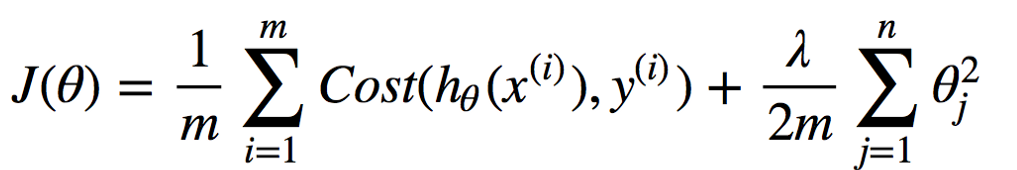
\includegraphics[width=.3\linewidth, height=1cm]{f2.png}
\end{center}
Where C is a complexity parameter, represented by $\alpha$ in sklearn, which also equals 1/2C.
The only difference between the four models trained is that they each have different C's: 1, 0.1, 0.01, 0.001. After training, the feature parameters were:
\begin{center}
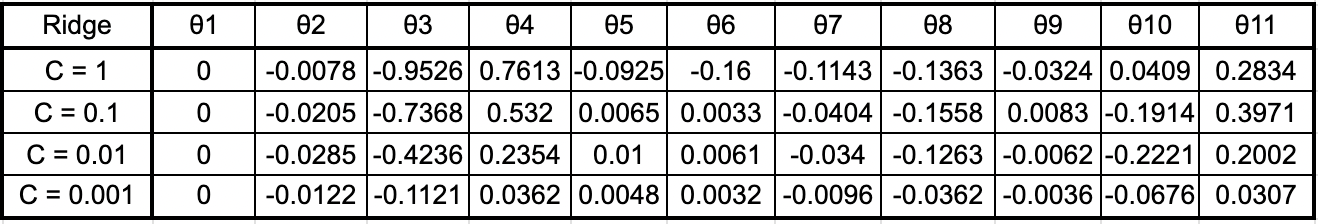
\includegraphics[width=\linewidth]{t3.png}
\caption{A table containing the Ridge feature parameters values for $\theta_1$  to  $\theta_{11}$  in the columns with each row representing a model with a different C value.}
\end{center}
\begin{center}
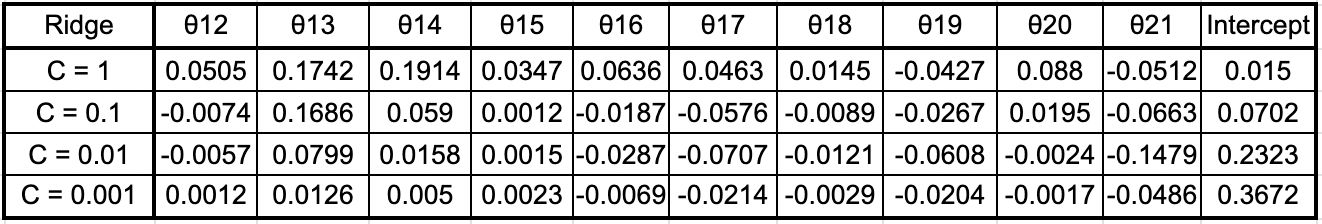
\includegraphics[width=\linewidth]{t4.png}
\caption{A table containing the Ridge feature parameters values for $\theta_12$  to  $\theta_{21}$ and the intercept in the columns with each row representing a model with a different C value.}
\end{center}

In the Ridge models as C gets bigger the feature parameters grow smaller. Unlike Lasso, as C gets larger the intercepts also get larger. The main difference between the two is the Ridge models have less parameters equal to 0 as Ridge Regression does not automatically eliminate the weight of features of lesser importance.

\begin{figure}
\centering
\begin{subfigure}{.5\linewidth}
  \centering
  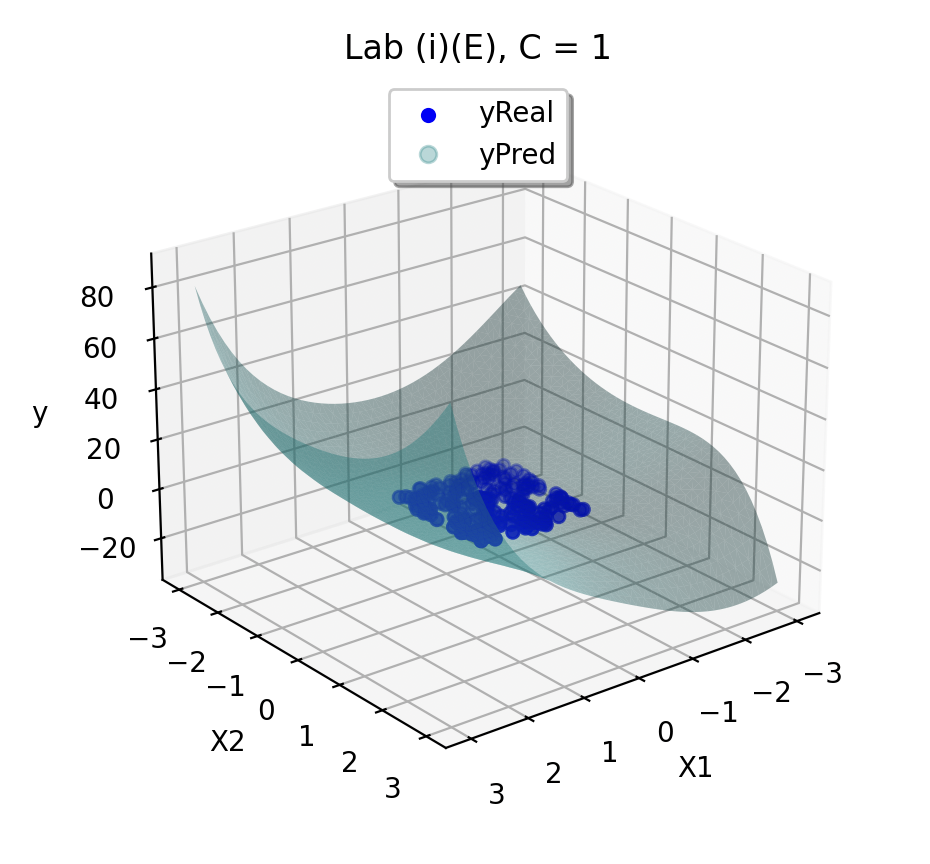
\includegraphics[width=\linewidth, height=8cm]{ie1.png}
  \caption{Ridge model predictions with C = 1}
  \label{fig:sub1}
\end{subfigure}%
\begin{subfigure}{.5\textwidth}
  \centering
  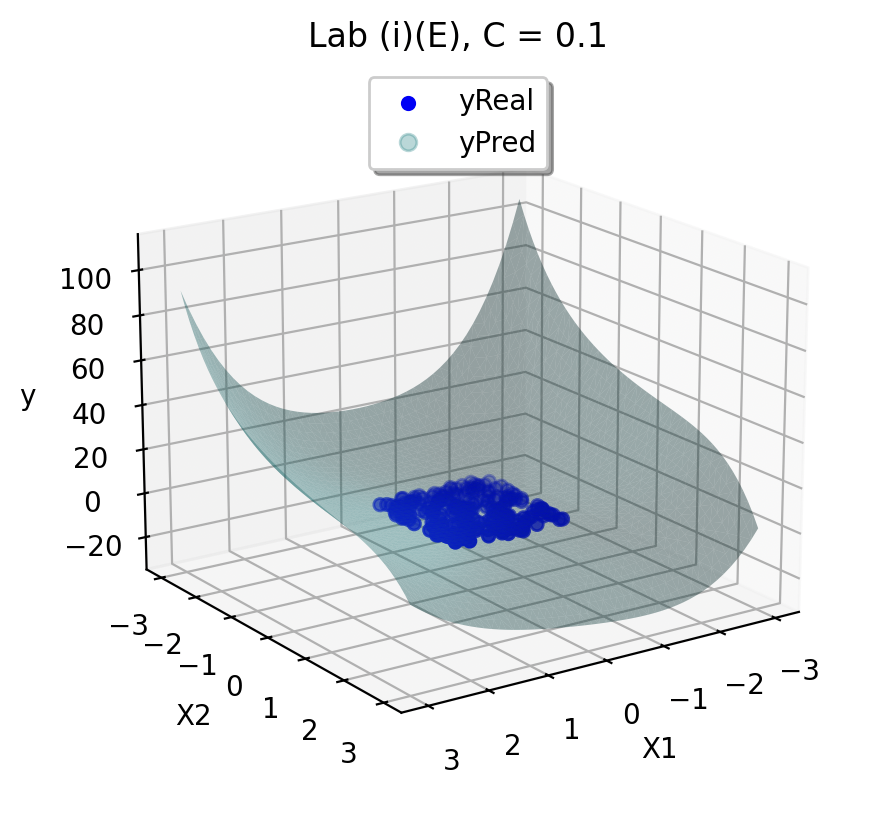
\includegraphics[width=\linewidth, height=8cm]{ie2.png}
  \caption{Ridge model predictions with C = 0.1}
  \label{fig:sub2}
\end{subfigure}
\label{fig:test}
\begin{subfigure}{.5\linewidth}
  \centering
  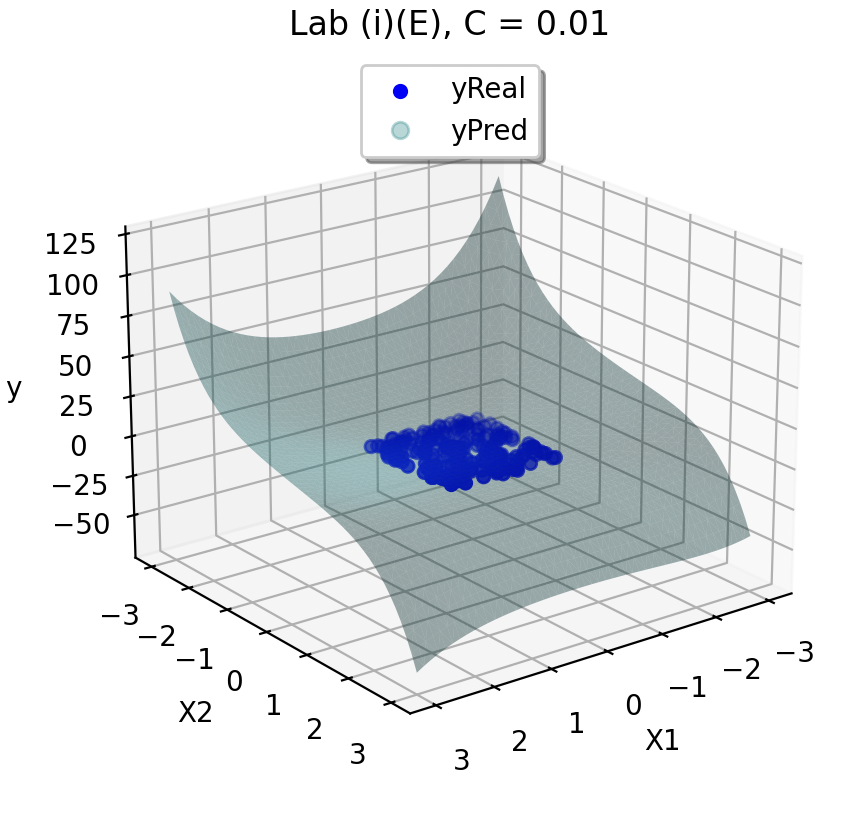
\includegraphics[width=\linewidth, height=8cm]{ie3.png}
  \caption{Ridge model predictions with C = 0.01}
  \label{fig:sub3}
\end{subfigure}%
\begin{subfigure}{.5\textwidth}
  \centering
  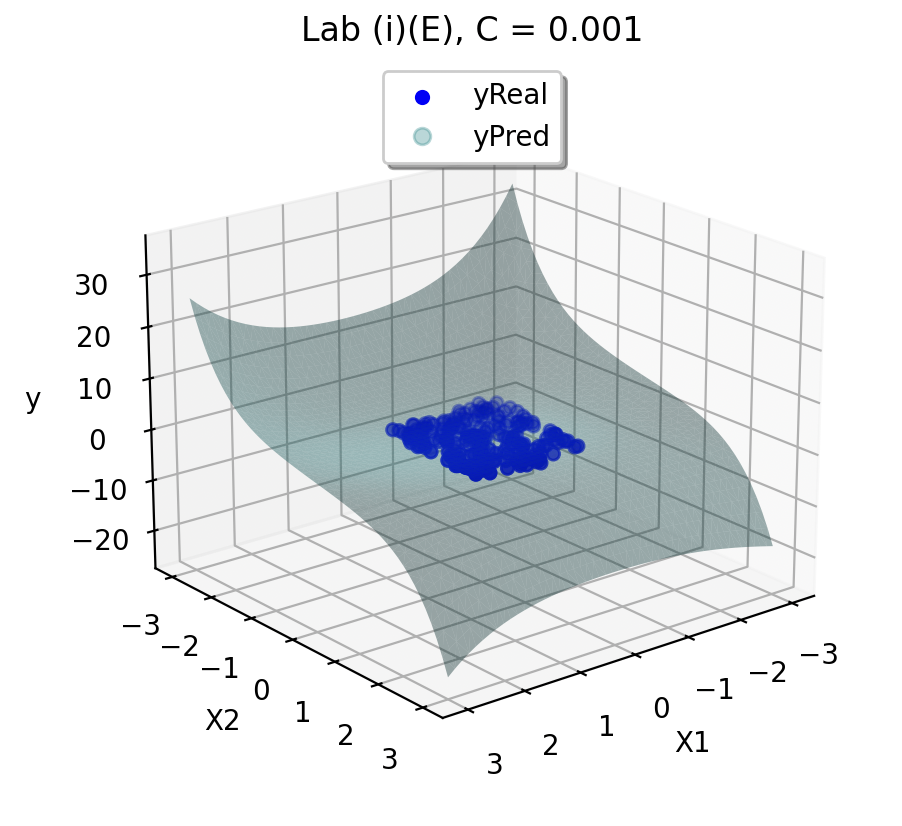
\includegraphics[width=\linewidth, height=8cm]{ie4.png}
  \caption{Ridge model predictions with C = 0.001}
  \label{fig:sub4}
\end{subfigure}
\caption{A figure with four subfigures, each containing a 3D scatter plot and plane that visualizes part ie of the lab.}
\label{fig:test}
\end{figure}

Again the models are tested using the same grid of X values from [-3,3] and plotted using a 3D surface, as seen in figure 7. The C value in ridge models controls the strength of the l2 penalty, as C increases the variance decreases and vice versa. The C also is in charge of keeping parameters small.

\section{Part ii}
\subsection{(ii)(a)}
We now perform K-fold Cross Validation on Lasso models in order to see what value of C is the best one to choose. We are using a 5-fold as specified in the instructions, so we split the data into five equal parts and train the model on four of these parts and then test on the final part. We repeat this until each part has had the chance to be the testing data. With each iteration we take the mean squared error of the predictions and once the iterations are done we calculated the mean of these mean squared errors and the standard deviation.

Then we repeat this for new models with different C values, the C values I chose for this cross validation are [0.1, 1, 10, 100, 1000]. I chose these values as they are the C values I used for my models in previous parts, plus 0.1 which I added to explore going even smaller. Also, these C's extend small enough and large enough to explore both underfitting and overfitting.

\subsection{(ii)(b)}
\begin{figure}
\centering
\begin{subfigure}{.5\linewidth}
  \centering
  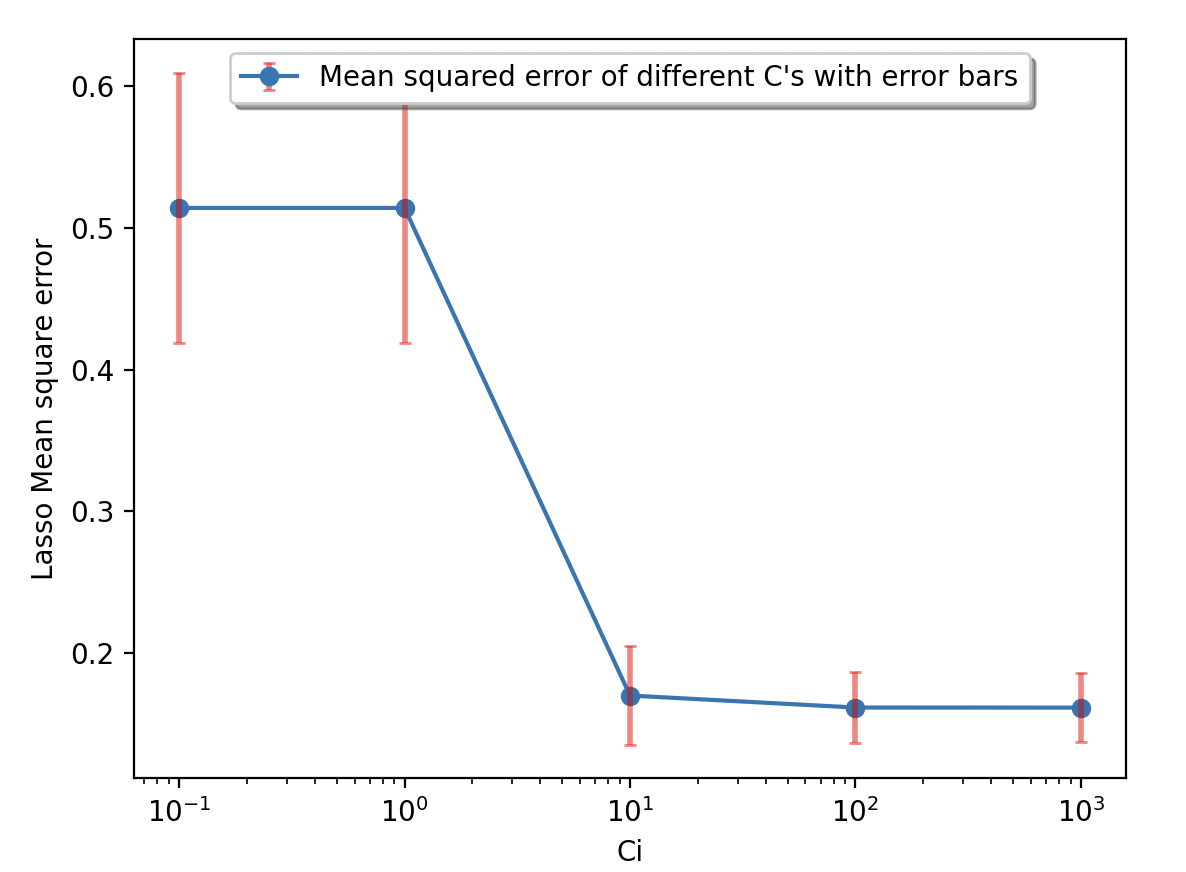
\includegraphics[width=\linewidth, height=8cm]{iia1.png}
  \caption{Lasso Cross Validation}
  \label{fig:sub1}
\end{subfigure}%
\begin{subfigure}{.5\textwidth}
  \centering
  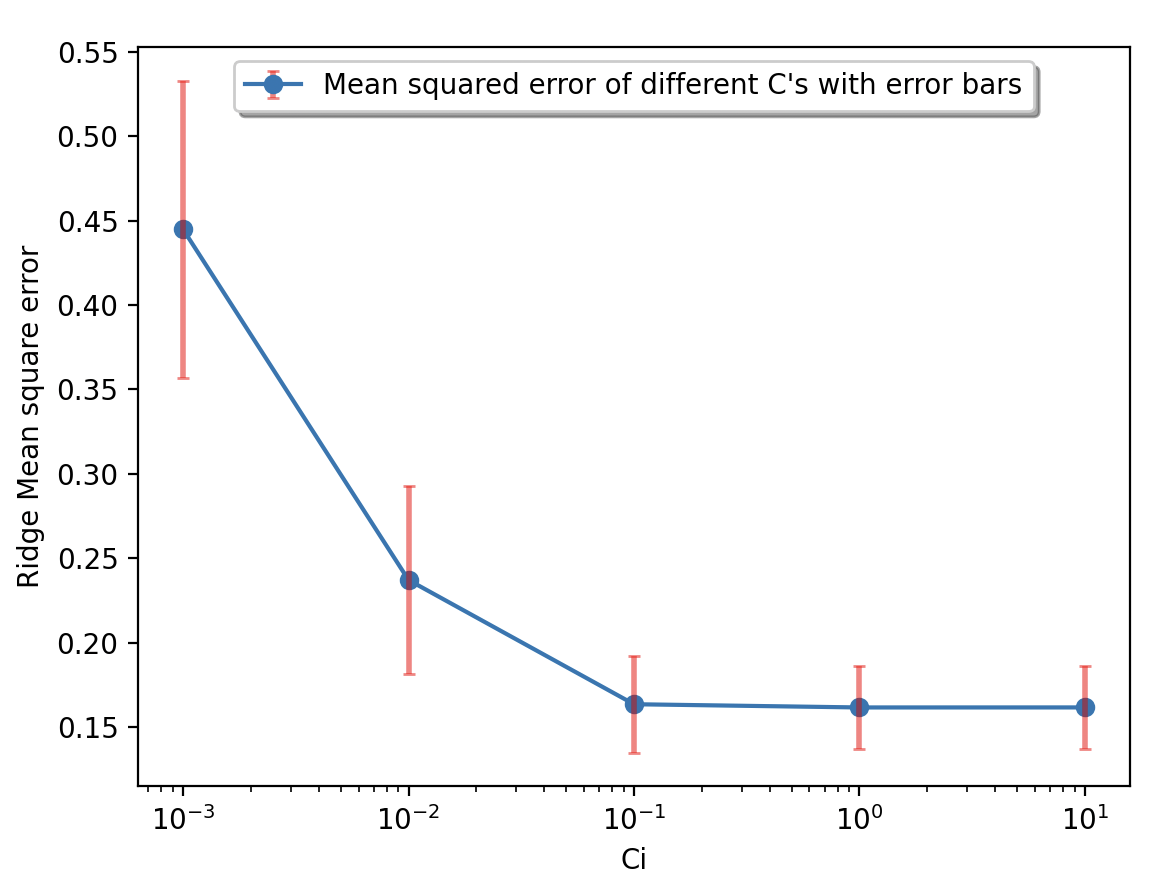
\includegraphics[width=\linewidth, height=8cm]{iia2.png}
  \caption{Ridge Cross Validation}
  \label{fig:sub2}
\end{subfigure}
\caption{A figure with two subfigures, each containing a mean error bar plot that visualizes part iia of the lab.}
\label{fig:test}
\end{figure}

Once we have the mean mean squared error and the standard deviation of these errors for each value of C, we then plot these means as points on a graph with the standard deviation creating an error bar.
In figure 8.a we see the results of our Lasso Cross Validation. We can see as C gets larger, our mean and standard deviation gets smaller. It's important to note that as C increases, $\alpha$ in sklearn decreases. From these results it looks like a C of 10 would be the best, as any lower and our mean error is too high as we are underfit while any higher will probably overfit our data. 

\subsection{(ii)(c)}
We then repeated the K-fold Cross Validation with Ridge Regression models and with different values of C. The values I chose for Ridge were [0.001, 0.01, 0.1, 1, 10]. I chose these values as they are the same as the ones used in my models from part ie with the addition of 10 to explore larger C's. Also because these represent a wide spread of C values that are both common and uncommon for Ridge models.

We see our Ridge cross validation results in figure 8.b. From this graph we can see that the best value of C for our Ridge model is 0.01 or 0.1, as any larger will probably overfit our data and any smaller will underfit as seen by the large mean errors and error bars. 



\section{Appendix}
\lstinputlisting[language=Python]{../main.py}
\end{document}



